\documentclass[12pt]{article}

\title{ET4340 Electronics for Quantum Computing\\Homework 3}
\author{
    Mick van Gelderen\\4091566
}
\date{November 2013}

\usepackage[utf8]{inputenc}
\usepackage[a4paper,margin=2.2cm]{geometry}
\usepackage{natbib}
\usepackage{graphicx}
\usepackage{listings}
\usepackage{framed}
\usepackage{mathtools}
\usepackage{braket}
\usepackage{ifmtarg}
\usepackage{multirow}

\newcommand{\pauli}[1]{
    \ensuremath{
        \begin{pmatrix}
            \if#1x
                0 & 1 \\
                1 & 0 \\
            \fi\if#1y
                0 & -i \\
                i & 0 \\
            \fi\if#1z
                1 & 0 \\
                0 & -1 \\
            \fi
        \end{pmatrix}
    }
}

\setlength{\parindent}{0cm}

\newcommand{\paulisigma}[1]{%
    \ensuremath{\sigma{}_{#1}}%
}

\newcommand{\pmat}[1]{\begin{pmatrix}#1\end{pmatrix}}
\newcommand{\rsqrt}[1]{\ensuremath{\frac{1}{\sqrt{#1}}}}

\setlength{\parskip}{0.5em plus4mm minus3mm}
\newenvironment{answer}{\begingroup\setlength{\leftskip}{-\leftmargin}\begin{framed}}{\end{framed}\endgroup}

\newcommand{\CNOT}[1]{\ensuremath{\texttt{CNOT}_{#1}}}
\newcommand{\CPHASE}[1]{\ensuremath{\texttt{CPHASE}_{#1}}}
\newcommand{\SWAP}[1]{\ensuremath{\texttt{SWAP}_{#1}}}
\newcommand{\cnotgr}[1]{\ensuremath{\pmat{%
        1 & 0 & 0 & 0 \\%
        0 & 1 & 0 & 0 \\%
        0 & 0 & 0 & 1 \\%
        0 & 0 & 1 & 0 \\%
}}}

\begin{document}

\maketitle
\hfill\\\\\\

\paragraph{Problem 1: Bell state analyzer} \hfill \\

In the previous homework, we introduced the \emph{Bell states}:

\begin{align*}
    \ket{\Psi_+} &= \rsqrt{2} (\ket{01} + \ket{10}) \\
    \ket{\Psi_-} &= \rsqrt{2} (\ket{01} - \ket{10}) \\
    \ket{\Phi_+} &= \rsqrt{2} (\ket{00} + \ket{11}) \\
    \ket{\Phi_-} &= \rsqrt{2} (\ket{00} - \ket{11}) \\
\end{align*}

Consider the quantum circuit below:

\begin{center}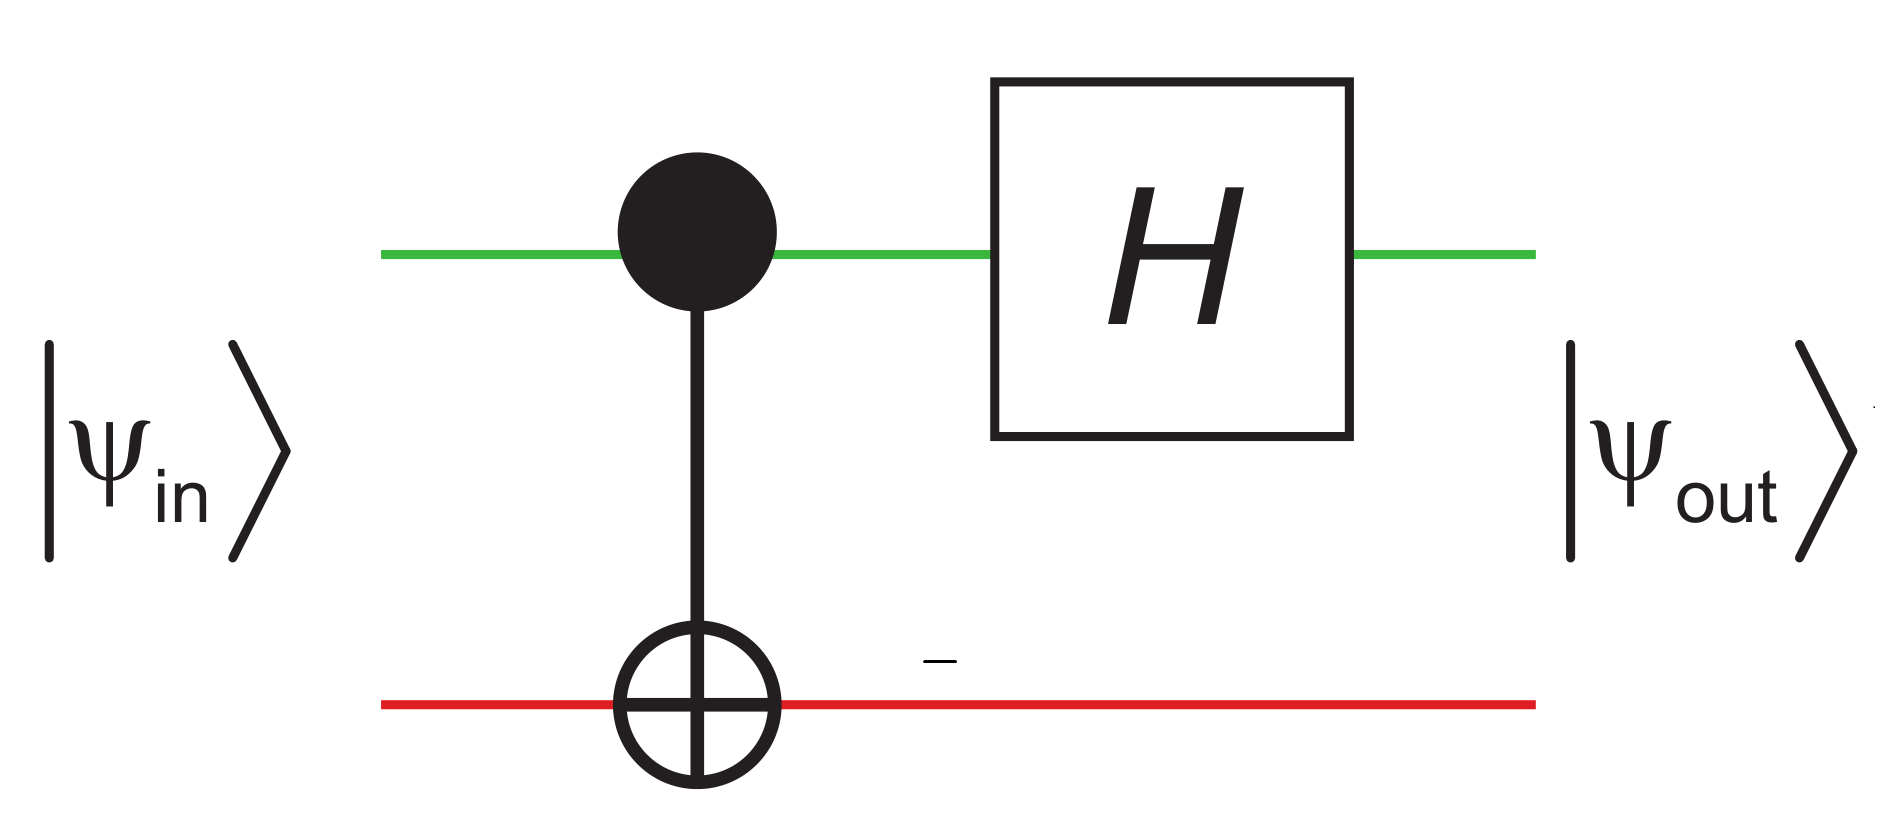
\includegraphics[width=.4\textwidth]{problem-1.png}\end{center}

\begin{enumerate}
    \item Give the $4 \times 4$ unitary matrix $T$ describing the transformation on the two qubits.

    \begin{answer}
        The transformation consists of a \CNOT{gr} followed by a Hadamard gate on the green qubit. The transformation matrix is found by computing $T = (H \otimes I)\CNOT{gr}$. Note that the order of the matrix combination is reversed with respect to the order they are in when you look at the circuit. This is only natural because we compute the output state $x^*$ of the input state $x$  as $x^* = Mx$ and not as $x^* = x^\dagger{}M$.

        \begin{align*}
            T &= \rsqrt{2}\pmat{1&0&1&0\\0&1&0&1\\1&0&-1&0\\0&1&0&-1}\cnotgr{} \\
            &= \rsqrt{2}\pmat{1&0&0&1\\0&1&1&0\\1&0&0&-1\\0&1&-1&0}
        \end{align*}
    \end{answer}

    \item Calculate the ouput state for each Bell state.

    \begin{answer}
        We simply apply $T$ to the Bell states one by one:

        \begin{alignat*}{3}
            T\ket{\Psi_+} &= \frac{1}{2}\pmat{1&0&0&1\\0&1&1&0\\1&0&0&-1\\0&1&-1&0}\pmat{0\\1\\1\\0}
                &= \frac{1}{2}\pmat{0\\2\\0\\0} &= \ket{01} \\
                \\
            T\ket{\Psi_-} &= \frac{1}{2}\pmat{1&0&0&1\\0&1&1&0\\1&0&0&-1\\0&1&-1&0}\pmat{0\\1\\-1\\0}
                &= \frac{1}{2}\pmat{0\\0\\0\\2} &= \ket{11} \\
                \\
            T\ket{\Phi_+} &= \frac{1}{2}\pmat{1&0&0&1\\0&1&1&0\\1&0&0&-1\\0&1&-1&0}\pmat{1\\0\\0\\1}
                &= \frac{1}{2}\pmat{2\\0\\0\\0} &= \ket{00} \\
                \\
            T\ket{\Phi_-} &= \frac{1}{2}\pmat{1&0&0&1\\0&1&1&0\\1&0&0&-1\\0&1&-1&0}\pmat{1\\0\\0\\-1}
                &= \frac{1}{2}\pmat{0\\0\\2\\0} &= \ket{10} \\
        \end{alignat*}

        Its also possible to reason what the outcomes will be. We will do this for a single Bell state to demonstrate this.

        Take the Bell state $\ket{\Psi_+}$. It consists of a combination of two computational basis components: $\ket{01}$ and $\ket{10}$. The effect of the \CNOT{gr} gate can be applied to these one by one. $\ket{01}$ is not changed because the control bit (or green bit) is $\ket{0}$. The other component $\ket{10}$ however becomes $\ket{11}$ because the control bit is $\ket{1}$ which causes the other bit to flip from $\ket{0}$ to $\ket{1}$. The combined state is now $\rsqrt{2}\left(\ket{01} + \ket{11}\right)$. We can write this as $\rsqrt{2}\left(\ket{0} + \ket{1}\right) \otimes \ket{1}$. This means that the green bit equals $\rsqrt{2}\left(\ket{0} + \ket{1}\right)$ and the red bit is $\ket{1}$. Now we apply the Hadamard gate to the green bit so that it becomes $\ket{0}$. The final state of the system is $\ket{0} \otimes \ket{1} = \ket{01}$. This result is ofcourse the same result as we got from the matrix multiplications.
    \end{answer}

    \item For each of the four Bell states, what will the outcomes be of measurements performed on the two qubits at the end?

    \begin{answer}
        Assuming we measure with respect to $Z$, we will always obtain the same measurement results, either $m = +1$ or $m = -1$, for each qubit since the Bell states produce a single computational state at the output. Repeating the experiment will always give $m = +1$ when measuring the green qubit for $\Psi_{in} = \Psi_+$ for example.
    \end{answer}

\end{enumerate}

\paragraph{Problem 2: Entanglement by measurement} \hfill \\

Consider the circuit below:

\begin{center}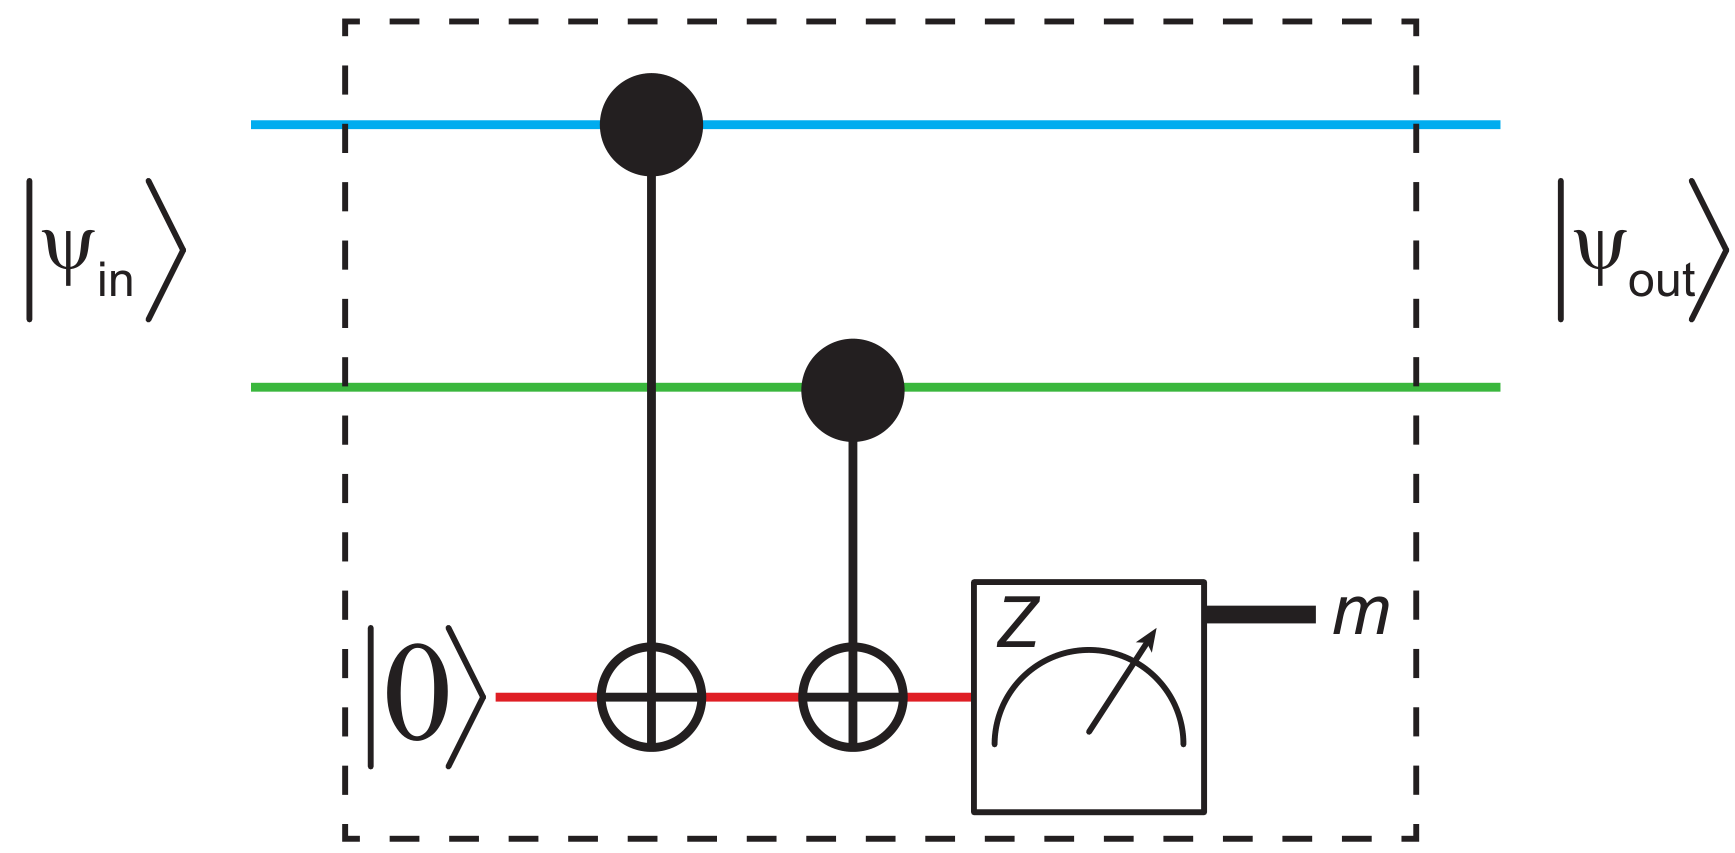
\includegraphics[width=.4\textwidth]{problem-2.png}\end{center}

The two input qubits are initially prepared in the maximal superposition state $\ket{\Psi} = \frac{1}{2}\left(\ket{00} + \ket{01} + \ket{10} + \ket{11}\right)$ and the ancilla qubit in $\ket{0}$.

\begin{enumerate}
    \item What is the state of the three-qubit system after the two \CNOT{} gates and before the measurement?

    \begin{answer}
        First of all, lets write the entire system as $\ket{\Psi_0} = \frac{1}{2}\left(\ket{000} + \ket{010} + \ket{100} + \ket{110}\right)$.
        After the first \CNOT{br} gate the system is in the state:
        \begin{align*}
            \ket{\Psi_1} = \frac{1}{2}\left(\ket{000} + \ket{010} + \ket{101} + \ket{111}\right)
        \intertext{Now we apply the second \CNOT{gr} gate}
            \ket{\Psi_2} = \frac{1}{2}\left(\ket{000} + \ket{011} + \ket{101} + \ket{110}\right)
        \end{align*}
        Both $\ket{\Psi_1}$ and $\ket{\Psi_2}$ are entangled states because they cannot be written as a product state.
    \end{answer}

    \item Using the generalized Born rule, find the probability of the ancilla measurement giving result $m = +1$.

    \begin{answer}
        Looking at $\ket{\Psi_2}$ I'd say that the ancilla bit has a $50\%$ chance to be measured as $m = +1$ since there are two kets with a $1$ and two with a $0$ at the end.

        If you apply $I \otimes I \otimes Z$ the resulting vector contains two $+1$'s and two $-1$'s which kind of strengthens my belief but I cannot give a sound reasoning.
    \end{answer}

    \item What is the final state of the two qubits when the ancilla measurement gives $m = +1$?

    \begin{answer}
        $\ket{\Psi_2}$ can be written as $\frac{1}{2}\left((\ket{00} + \ket{11})\otimes\ket{0} + (\ket{01} + \ket{10})\otimes\ket{1}\right)$. If the measurement is $m = +1$, the ancilla qubit is in the state $\ket{0}$ so the other two qubits are in $\rsqrt{2}(\ket{00} + \ket{11})$ which is the Bell state $\ket{\Phi_+}$.
    \end{answer}

    \item What is the final state of the two qubits when the ancilla measurement gives $m = -1$?

    \begin{answer}
        The Bell state $\ket{\Psi_+}$.
    \end{answer}

    \item Suppose that when $m = -1$, and only then, you apply $X$ to one of the qubits (this implements a form of feedback control). What will the final state be in this case?

    \begin{answer}

    \end{answer}
\end{enumerate}
\end{document}

